\section{Polynomial-time algorithm for \onewriter\ systems}
\label{sec:onewriter}

We now consider programs where, for every variable, there is a single thread which writes to it. Any number of threads can read from a variable. An execution graph $\ex = \tuple{\E, \po, \rf, \mo}$ is said to be a \onewriter\ execution graph if for each memory location $x$, the entire set of its write events $\W_x$ belong to one thread. 

\noindent \textbf{Overview of this section.} The fact that we work with \onewriter\ execution graphs simplifies several axioms of Table~\ref{table:ax:models-2}, allowing for  a polynomial-time procedure. Recall however that for sequential consistency, the \onewriter\ assumption offers no specific advantage and still yields a $\NP$-hard complexity~\cite{gibbons}. 

\noindent \textit{$\sramm$ and $\ramm$ reduce to $\wramm$.} Firstly, we note that consistency checking for the $\sramm$ and $\ramm$ memory models reduce to checking for $\wramm$ in \onewriter\ execution graphs (Lemma~\ref{lem:one-writer-reduces-to-wra}). Moreover, since all writes of a memory location lie in a single thread, the $\mo$ relation on writes gets fixed to the unique order that agrees with $\po$.  Therefore, the problem boils down to detecting if there is an $\rf$ that satisfies \emph{porf-acyclicity} and \emph{weak-read-coherence}, the two axioms needed for $\wramm$ consistency. So we focus on these two axioms for the rest of the section. 

\noindent \textit{A partial order on $\rf$.} Secondly, since all writes to a memory location $x$ are totally ordered by $\po$, there is a natural partial order induced on the $\rf$ relations. A reads-from relation $\rf_1$ is said to be smaller than $\rf_2$, written as $\rf_1 \sqsubseteq \rf_2$, if for every 
read $r$, the write event $w_2 = \rf^{-1}_2(r)$ appears $\po$-later than $w_1 = \rf^{-1}_1(r)$ (we say $w_2$ is $\po$-later than $w_1$ if $w_1~\po^*w_2$). In other words, $\rf_2$ associates each read $r$ to a write that appears later in the program order compared to the write that $\rf_1$ associates it to\label{order}. %%%%%%% 
We observe two useful properties of this partial order: (1) if an $\rf$ violates porf-acyclicity, then every $\rf^{\dagger}$ larger than it also violates porf-acyclicity, and (2) among all the $\rf$ that satisfy weak-read-coherence, there is a unique minimum element $\rf_{\min}$.

\noindent \textit{Algorithm.} Using these two properties, we design an algorithm that starts with the smallest $\rf$ and iteratively computes larger reads-from relations until a $\wramm$-consistent $\rf$ is found. If this $\rf$ additionally satisfies porf-acyclicity, we have found a reads-from relation that witnesses the $\wramm$-consistency. Else, we conclude that no such $\rf$ exists.  

The two useful properties appear in Section~\ref{sec:onewriter-structural-properties} and the algorithm is described in Section~\ref{sec:onewriter-algorithm}. Section~\ref{sec:1-writer-hardness} presents a lower bound for \onewriter\ systems.

\subsection{Structural properties of \onewriter\ execution graphs}
\label{sec:onewriter-structural-properties}
Our first observation is that for \onewriter\ systems, checking $\sramm$ and $\ramm$ reduces to checking $\wramm$.  For $\wramm$ the only axioms are porf-acyclicity and weak-read-coherence.  For $\ramm$ one must also ensure write-coherence and read-coherence, in addition to porf-acyclicity.  In a \onewriter\ setting, write-coherence is enforced by choosing $\mo$ to agree with $\po$ (so all writes to a location are ordered by the program order of their single writer).  

A violating cycle for read-coherence has the form
\[
\rd(x) \xra{\rf^{-1}} \wt(x) \xra{\mo_x} \wt'(x) \xra{\hb} \rd(x).
\]
When $\mo$ agrees with $\po$, the $\mo_x$ edge is simply $\po^+$, since both $\wt_x$ and $\wt'_x$ are in the same thread. Now, a violating cycle for weak-read-coherence has the form
\[
\rd(x) \xra{\rf^{-1}} \wt(x) \xra{\hb} \wt'(x) \xra{\hb} \rd(x),
\]
and, since $\wt(x)$ and $\wt'(x)$ come from the same thread, the $\hb$ step between $\wt(x)$ and $\wt'(x)$ can likewise be instantiated by $\po^+$.  Hence read-coherence coincides with weak-read-coherence in the \onewriter\ setting.  Moreover, having an $\mo$ agreeing with $\po$ reduces strong-write-coherence to porf-acyclicity, culminating in this lemma.  

\begin{restatable}{lemma}{lemonewriterreducestowra}
    \label{lem:one-writer-reduces-to-wra}
 Let $\ex = \tuple{\E, \po, \rf, \mo}$ be a \onewriter\ execution graph. Then, for $\MemModel \in \{\sramm, \ramm\}$, we have $\ex \models \MemModel$ iff $\mo$ agrees with $\po$ and $\ex \models \wramm$. 
\end{restatable}
\begin{proof}
    Let us begin with $\MemModel = \ramm$. For $\ex$ to be consistent with $\ramm$, it has to satisfy the three axioms: porf-acyclicity, write-coherence and read-coherence~(see Table~\ref{table:ax:models-2}). In a \onewriter\ system, for $\mo$ edges, both its source and target are in the same thread. Therefore, to satisfy write-coherence, $\mo$ should agree with $\po$: in other words, if $w_1~\mo_x~w_2$, then $w_1~\po^+~w_2$. Hence, notice that to prove the lemma, it is sufficient to show that the read-coherence axiom and weak-read-coherence axiom coincide for \onewriter. A violating cycle for read-coherence is of the form
    \[r \xra{\rf} w_1 \xra{\mo_x} w_2 \xra{\hb} r\]
    As seen above the $\mo_x$ edge is simply $\po^+$, hence $w_1 \xra{\mo_x} w_2$ can be replaced with $w_1 \xra{\po^+} w_2$. A violating cycle for weak-read-coherence is of the form
    \[r \xra{\rf} w_1 \xra{\hb} w_2 \xra{\hb} r\]
    with $w_1$ and $w_2$ being writes on the same variable $x$. Since the writes are on the same variable, $w_1 \xra{\hb} w_2$ can be replaced with $w_1 \xra{\po^+} w_2$. This proves that the violating cycles for both the axioms coincide for \onewriter\ systems.

    Now, let $\MemModel = \sramm$. For strong-write-coherence to be true, we require $\mo$ to agree with $\po$. If $X \models \sramm$, then the axioms porf-acyclicity, strong-write-coherence and read-coherence are true. Since strong-write-coherence holds, $\mo$ needs to agree with $\po$. We have shown above that read-coherence coincides with weak-read-coherence, when $\mo$ agrees with $\po$. Hence $X \models \wramm$. Now, for the other direction. Suppose $\mo$ agrees with $\po$ and weak-read-coherence are true. From above, we deduce read-coherence holds. If strong-write-coherence is violated, then there will be a porf-cycle, a contradiction. Hence, the lemma follows for $\MemModel = \sramm$.
\end{proof}
As a consequence, the consistency checking of \onewriter\ under $\sramm$, $\ramm$ and $\wramm$ boils down to checking porf-acyclicity and weak-read-coherence violations.
Secondly, the problem of synthesizing both $\rf$ and $\mo$ boils down to just synthesizing $\rf$, since $\mo$ is fixed to the order that respects $\po$. Nevertheless, there are still exponentially many $\rf$ relations possible. The next lemma entails that there is a ``smallest'' $\rf$ among all $\wramm$-consistent $\rf$s in the $\sqsubseteq$ order on $\rf$s defined in the overview of this section. Given $\rf_1, \rf_2$, we write $\min(\rf_1, \rf_2)$ for the reads-from relation which associates every read $r$ to the $\po$-smaller write between $\rf^{-1}_1(r)$ and $\rf^{-1}_2(r)$.


\begin{restatable}{lemma}{lemmaonewritertwoproperties}
    \label{lem:onewriter-axioms-two-properties}
Let $\rf_1$ and $\rf_2$ be two reads-from relations over a partial \onewriter\ execution graph $\ex=\tuple{\E, \po, \mo}$ s.t. $\mo$ agrees with $\po$. 
\begin{itemize}
\item Suppose $\rf_1 \sqsubseteq \rf_2$. Then, if $\rf_1$ induces a $\po \cup \rf_1$ cycle, then $\rf_2$ induces a $\po \cup \rf_2$ cycle.
\item Suppose both $\rf_1$ and $\rf_2$ satisfy weak-read-coherence. Then,  $\min(\rf_1, \rf_2)$ also satisfies weak-read-coherence.
\end{itemize} 
\end{restatable}
\begin{proof}
For the first item, suppose $\rf_1$ induces a porf-cycle of the form:
\[ e_1 \xra{\rf_1} f_1 \xra{\po} e_2 \xra{\rf_1} f_2 \cdots e_m \xra{\rf_1} f_{m} \xra{\po} e_1\]
Notice that each $e_i$ is a write event and $f_i$ is a read event such that $e_i = \rf_1(f_i)$. Since $\rf_1 \sqsubset \rf_2$, we know $\rf_1(f_i) \xra{\po^*} \rf_2(f_i)$. Hence: $e_i \xra{\po^*} e'_i$ where $e'_i = \rf_2(f_i)$. This gives the following $\po \cup \rf_2$ cycle:
 \[ e_1 \xra{\po^*} e'_1 \xra{\rf_2} f_1 \xra{\po} e_2 \xra{\po^*} e'_2 \xra{\rf_2} f_2 \cdots e_m \xra{\po^*} e'_m \xra{\rf_2} f_{m} \xra{\po} e_1\]
 This proves the first item.

 For the second item, denote $\rf_0 = \min(\rf_1, \rf_2)$. We will show that if $\rf_0$ violates weak-read-coherence, then either $\rf_1$ or $\rf_2$ violates it. Suppose $\rf_0$ induces a violation of weak-read-coherence. There is a cycle of the form:
 \[ r \xra{\rf_0^{-1}} w \xra{\po^+} w' \xra{\hb_0} r \]
 where both $w$ and $w'$ are on the same variable, and hence the edge between them is $\po^+$. By definition, either $\rf_1$ or $\rf_2$ associates $r$ to $w$. Let us say $\rf_1(r) = w$. If we show $w' \hb_0 r$ then we are done. Since $w'~\hb_0~r$, there is a path with $\po$ and $\rf_0$ edges from $w'$ to $r$:
 \[w' \xra{\po^*} e_1 \xra{\rf_0} f_1 \xra{\po^*} e_2 \xra{\rf_0} f_2 \cdots e_m \xra{\rf_0} f_m \xra{\po^*} r \]
 We will now form a $\po \cup \rf_1$ path from $w'$ to $r$. For each $e_i \xra{\rf_0} f_i$, either $e_i \xra{\rf_1} f_i$ too, in which case we retain that edge. If not, by construction of $\rf_0$, we know that $e_i \xra{\rf_2} f_i$ and $e_i \po^* \rf_1(f_i)$. Replace $e_i \xra{\rf_0} f_i$ by the sequene $e_i \po^* \rf_1(f_i) \xra{\rf_1} f_i$ as in the proof of the first item, to deduce an $\hb_1$ path from $w'$ to $r$. This show that there is a violating cycle for weak-read-coherence induced by $\rf_1$ too, thereby proving the second item. 
\end{proof}
Suppose $S$ is the set of all $\rf$ that satisfy weak-read-coherence. The second item of Lemma~\ref{lem:onewriter-axioms-two-properties} implies that $S$ contains a unique minimum element, which we denote by $\rf_{\min}$. By the first item of Lemma~\ref{lem:onewriter-axioms-two-properties}, if $\rf_{\min}$ violates porf-acyclicity then every $\rf$ in $S$ also violates it. Therefore, $\wramm$-consistency checking reduces to computing $\rf_{\min}$ and testing it for porf-acyclicity. The algorithm in the next section performs exactly this construction and test. 

\begin{figure}[!tbp]
   \def\ystep{0.5}

\centering
	\scalebox{.7}{
\begin{tikzpicture}[yscale=1]
\node (t01) at (-.2, 1.5*\ystep) {$t_1$};
\node (t02) at (1.5, 1.5*\ystep) {$t_2$};
\node (t03) at (3, 1.5*\ystep) {$t_3$};

  \node (t11) at (-.2, 0*\ystep) {$\wt_1(x,1)$};
    \node (t12) at (1.5, 0*\ystep) {$\rd_1(x,2)$};
    \node (t13) at (3, 0*\ystep) {$\rd_2(y,1)$};
    
    
    \node (t21) at (-.2, -2*\ystep) {$\wt_2(x,2)$};
    \node (t22) at (1.5, -2*\ystep) {$\rd_3(x,1)$};    
    
    \node (t23) at (3, -2*\ystep) {$\rd_4(x,2)$};
    
    
    \node (t31) at (-.2, -4*\ystep) {$\wt_3(x,1)$};
    \node (t32) at (1.5, -4*\ystep) {$\wt_4(y,1)$};
    
    \node (t41) at (-.2, -6*\ystep) {$\wt_5(x,2)$};
    
    \node (n1) at (1.5,-8*\ystep) {$\rf_0$};
    
    \draw[po] (t11) -- (t21);
    \draw[po] (t21) -- (t31);
    \draw[po] (t31) -- (t41);
    
    \draw[po] (t12) -- (t22);
    \draw[po] (t22) -- (t32);
    \draw[po] (t13) -- (t23);
    
      
    \draw[rf] (t11) -- (t22);
    \draw[rf] (t21) -- (t12);
    \draw[rf] (t21) to[out=-25,in=-160] (t23);
    \draw[rf] (t32) -- (t13);
    
    %%%%rf_0%%%%
    \node (t01) at (5, 1.5*\ystep) {$t_1$};
\node (t02) at (6.5, 1.5*\ystep) {$t_2$};
\node (t03) at (8, 1.5*\ystep) {$t_3$};

  \node (t11) at (5, 0*\ystep) {$\wt_1(x,1)$};
    \node (t12) at (6.5, 0*\ystep) {$\rd_1(x,2)$};
    \node (t13) at (8, 0*\ystep) {$\rd_2(y,1)$};
    
    
    \node (t21) at (5, -2*\ystep) {$\wt_2(x,2)$};
    \node (t22) at (6.5, -2*\ystep) {$\rd_3(x,1)$};   
    \node (t23) at (8, -2*\ystep) {$\rd_4(x,2)$};
    
    
    \node (t31) at (5, -4*\ystep) {$\wt_3(x,1)$};
    \node (t32) at (6.5, -4*\ystep) {$\wt_4(y,1)$};
    
    \node (t41) at (5, -6*\ystep) {$\wt_5(x,2)$};
    
    \node (n1) at (6.5,-8*\ystep) {$\rf_1$};
    
    \draw[po] (t11) -- (t21);
    \draw[po] (t21) -- (t31);
    \draw[po] (t31) -- (t41);
    
    \draw[po] (t12) -- (t22);
    \draw[po] (t22) -- (t32);
    \draw[po] (t13) -- (t23);
    
      
    \draw[rf] (t31) -- (t22);
    \draw[rf] (t21) -- (t12);
    \draw[rf] (t21) to[out=-25,in=-160] (t23);
    \draw[rf] (t32) -- (t13);
    
    %%%%rf_1%%%%
    
    \node (t01) at (10, 1.5*\ystep) {$t_1$};
\node (t02) at (11.5, 1.5*\ystep) {$t_2$};
\node (t03) at (13, 1.5*\ystep) {$t_3$};

  \node (t11) at (10, 0*\ystep) {$\wt_1(x,1)$};
    \node (t12) at (11.5, 0*\ystep) {$\rd_1(x,2)$};
    \node (t13) at (13, 0*\ystep) {$\rd_2(y,1)$};
    
    
    \node (t21) at (10, -2*\ystep) {$\wt_2(x,2)$};
    \node (t22) at (11.5, -2*\ystep) {$\rd_3(x,1)$};   
    \node (t23) at (13, -2*\ystep) {$\rd_4(x,2)$};
    
    
    \node (t31) at (10, -4*\ystep) {$\wt_3(x,1)$};
    \node (t32) at (11.5, -4*\ystep) {$\wt_4(y,1)$};
    
    \node (t41) at (10, -6*\ystep) {$\wt_5(x,2)$};
    
    \node (n1) at (11.5,-8*\ystep) {$\rf_2$};
    
    \draw[po] (t11) -- (t21);
    \draw[po] (t21) -- (t31);
    \draw[po] (t31) -- (t41);
    
    \draw[po] (t12) -- (t22);
    \draw[po] (t22) -- (t32);
    \draw[po] (t13) -- (t23);
    
      
    \draw[rf] (t31) -- (t22);
    \draw[rf] (t21) -- (t12);
    \draw[rf] (t41) to[out=-15,in=250] (t23);
    \draw[rf] (t32) -- (t13);

     \end{tikzpicture}}
     


\caption{\footnotesize From left: $\rf_0 \sqsubseteq \rf_1 \sqsubseteq \rf_2$. $\rf_0$ has a violation of \WRCoh{}:~$\rd_3 \xra{\rf_{0}^{-1}} \wt_1 \xra{\po} \wt_2 \xra{\hb_0} \rd_3 $.  $\rf_1$ has a violation of \WRCoh{}:~$\rd_4 \xra{\rf_{1}^{-1}} \wt_2 \xra{\po} \wt_3 \xra{\hb_1} \rd_4 $. $\rf_2$ does not have any more violations of \WRCoh{}. \PORF{} is also satisfied by $\rf_2$. The underlying partial execution graph is $\wramm$-consistent.
}\label{Example-one-writer-without-porfcycle}

\end{figure}

\subsection{Algorithm}
\label{sec:onewriter-algorithm}

Our algorithm starts from an $\rf_0$ which maps every read $r$ to the $\po$-smallest  write in its writer thread, such that the value of the chosen write matches with that of $r$, and in case the writer thread is the same as the one where $r$ is present, the mapped write lies above $r$. This relation $\rf_0$ may not satisfy weak-read-coherence. In that case, a violating cycle is identified and $\rf_0$ is modified to $\rf_1$ as explained below. Assume we have iteratively constructed upto $\rf_i$, and $\rf_i$ does not satisfy weak-read-coherence.  



%\begin{wrapfigure}[20]{r}{0.4\textwidth}
   
\begin{figure} 
  \def\ystep{0.5}
\centering
	\scalebox{.7}{
\begin{tikzpicture}[yscale=1]
\node (t01) at (-.2, 1.5*\ystep) {$t_1$};
\node (t02) at (1.5, 1.5*\ystep) {$t_2$};

  \node (t11) at (-.2, 0*\ystep) {$\wt_1(x,1)$};
    \node (t12) at (1.5, 0*\ystep) {$\rd_1(x,2)$};
    
    \node (t21) at (-.2, -2*\ystep) {$\wt_2(x,2)$};
    \node (t22) at (1.5, -2*\ystep) {$\rd_3(x,1)$};    
    
    \node (t31) at (-.2, -4*\ystep) {$\rd_2(y,1)$};
    \node (t32) at (1.5, -4*\ystep) {$\wt_4(y,1)$};
    
    \node (t41) at (-.2, -6*\ystep) {$\wt_5(x,1)$};
    
    \node (n1) at (1.1,-8*\ystep) {$\rf_0$};
    
    \draw[po] (t11) -- (t21);
    \draw[po] (t21) -- (t31);
    \draw[po] (t31) -- (t41);
    
    \draw[po] (t12) -- (t22);
    \draw[po] (t22) -- (t32);
      
    \draw[rf] (t21) to (t12);
    \draw[rf] (t11) -- (t22);
    \draw[rf] (t32) to (t31);
    \node (t01) at (4, 1.5*\ystep) {$t_1$};
\node (t02) at (5.5, 1.5*\ystep) {$t_2$};

  \node (t11) at (4, 0*\ystep) {$\wt_1(x,1)$};
    \node (t12) at (5.5, 0*\ystep) {$\rd_1(x,2)$};
    
    \node (t21) at (4, -2*\ystep) {$\wt_2(x,2)$};
    \node (t22) at (5.5, -2*\ystep) {$\rd_3(x,1)$};   
    
    \node (t31) at (4, -4*\ystep) {$\rd_2(y,1)$};
    \node (t32) at (5.5, -4*\ystep) {$\wt_4(y,1)$};
    
    \node (t41) at (4, -6*\ystep) {$\wt_5(x,1)$};
    
    \node (n1) at (5.2,-8*\ystep) {$\rf_1$};
    
     \draw[po] (t11) -- (t21);
    \draw[po] (t21) -- (t31);
    \draw[po] (t31) -- (t41);
    
    \draw[po] (t12) -- (t22);
    \draw[po] (t22) -- (t32);
    
    \draw[rf] (t21) to (t12);
    \draw[rf] (t41) to[out=30,in=-135] (t22);
    \draw[rf] (t32) to (t31);
    
    \end{tikzpicture}}
     


\caption{\footnotesize From left: $\rf_0 \sqsubseteq \rf_1$. $\rf_0$ has a violation of \WRCoh{}:~$\rd_3 \xra{\rf_{0}^{-1}} \wt_1 \xra{\po} \wt_2 \xra{\hb} \rd_3 $.  $\rf_1$ has no \WRCoh{} violation but does not satisfy \PORF{}:~$\wt_5 \xra{\rf_{1}} \rd_3 \xra{\po} \wt_4 \xra{\rf} \rd_2 \xra{\po} \wt_5$. The partial execution graph is not $\wramm$-consistent.
}\label{Example-one-writer-with-porfcycle}  
\end{figure}

\noindent \emph{From $\rf_i$ to $\rf_{i+1}$.} Pick a violating cycle for weak-read-coherence:
\[ r_i \xra{\rf_{i}^{-1}} w_i \xra{\hb_i} w'_i \xra{\hb_i} r_i \]
where all three events $r_i, w_i, w'_i$ are over the same variable, say $x_i$, and $\hb_i$ is $(\po \cup \rf_i)^+$. Recall that since we are in the \onewriter\ case, the intermediate $\hb_i$ can be replaced with $\po^+$. Modify $\rf_i$ to eliminate the violating cycle: choose a write for $r_i$ which appears on or after $w'_i$, that is, pick $w''_i$ such that $w'_i~\po^* w''_i$ and $w''_i$ is a write on the same variable $x_i$, writing the same value as the read event $r_i$. If no such write exists, conclude that there is no $\rf$ for $\expartial$ that satisfies weak-read-coherence. Else, let the resulting $\rf$ be called $\rf_{i+1}$. If $\rf_{i+1}$ does not satisfy weak-read-coherence, we update $\rf_{i+1}$ as above. Else, $\rf_{i+1}$ satisfies weak-read-coherence. We declare $\rf_{\min} = \rf_{i+1}$.

Finally, we test whether $\rf_{\min}$ satisfies porf-acyclicity. If it does, we have a witness for $\wramm$-consistency. Else, we conclude (due to Lemma~\ref{lem:onewriter-axioms-two-properties}) that $\expartial$ is not $\wramm$-consistent. 
We formalize this discussion in Algorithm~\ref{algo:one-writer-wra}. Here is the key invariant maintained by the algorithm: at each step $i$ where the update function is called on $\rf_i$,  we can show that $\rf_i \sqsubseteq \rf^{\dagger}$ for every $\rf^\dagger$ that satisfies weak-read-coherence. Figures~\ref{Example-one-writer-without-porfcycle} and ~\ref{Example-one-writer-with-porfcycle} illustrate the running of the algorithm on two different partial execution graphs. 





\begin{algorithm}[h!]
\caption{$\wramm$-consistency checking in \onewriter\ systems}
\label{algo:one-writer-wra}
\Fn{$\CheckC(\expartial)$}{
    $\rf \gets \Initialize(\expartial)$ \\
    \While{$\rf$ violates weak-read-coherence}{\label{algo-while-main-onewriter}
        $\rf \gets \update(\expartial, \rf)$  \label{algo-update-call}
    }
    \Comment{Now $\rf = \rf_{\min}$}
    \If{$\rf$ satisfies porf-acyclicity}{ \label{algo-check-porf}
        \Return $\expartial$ is $\wramm$-consistent \label{algo-declare-consistent}
    }
    \Else {
        \Return $\expartial$ is not $\wramm$-consistent  \label{algo-porf-cycle}
    }
}


\Fn{$\Initialize(\expartial)$}{
\For{each read $r = \rd(x, v)$}{
$t \gets$  thread containing $r$ \\
$t_x \gets$ writer thread for $x$ \\
\If{$t \neq t_x$}{
    $\rf^{-1}_0(r) \gets$ $\po$-smallest write $w$ of the form $\wt(x,v)$ in $t_x$ \\
    \If{there is no such write}{
        \Return $\expartial$ is not $\wramm$-consistent \label{init-not-consistent1}
    }
}
\If{$t = t_x$}{
    $\rf^{-1}_0(r) \gets$ $\po$-smallest write $w$ of the form $\wt(x,v)$ in $t_x$ s.t. $w~\po^+r$ \\
    \If{there is no such write}{
        \Return $\expartial$ is not $\wramm$-consistent \label{init-not-consistent2}
    }
}
}
\Return $\rf_0$
}

\Fn{$\update(\expartial, \rf_i)$}{
    Pick a cycle violating weak-read-coherence: $r_i \xra{\rf_i^{-1}} w_i \xra{\hb_i} w'_i \xra{\hb_i} r_i$ \label{algo-violatecycle} \\
    Let $r_i = \rd(x, v)$, $w_i = \wt(x, v)$, $w'_i = \wt(x, v')$ \\
    $t \gets$ thread of $r_i$ \\
    $t_x \gets$ writer thread of variable $x$ \\
    \If{$t \neq t_x$}{
    $\rf^{-1}_{i+1}(r_i) \gets$ $\po$-smallest write $w''_i$ of the form $\wt(x,v)$ in $t_x$ s.t. $w'_i ~\po* w''_i$ \label{algo-update1} \\
    \If{there is no such write}{
        \Return $\expartial$ is not $\wramm$-consistent  \label{algo-update-notconsistent1}
    }
}
\If{$t = t_x$}{
    $\rf^{-1}_{i+1}(r_i) \gets$ $\po$-smallest write $w''_i$ of the form $\wt(x,v)$ in $t_x$ s.t. $w'_i ~\po^* w''_i ~\po^+r_i$ \label{algo-update2}\\
    \If{there is no such write}{
        \Return $\expartial$ is not $\wramm$-consistent \label{algo-update-notconsistent2}
    }
}
$\rf^{-1}_{i+1}(r') \gets \rf_i(r')$ for all $r' \neq r_i$ \\
\Return $\rf_{i+1}$
}
\end{algorithm}

\begin{restatable}{theorem}{thmwracorrectness}
A partial execution graph $\expartial = \tuple{\E, \po}$ of a one-writer system is consistent for $\wramm$ iff Algorithm~\ref{algo:one-writer-wra} returns $\expartial$ is $\wramm$-consistent. Moreover, the algorithm runs in time $\mathcal{O}(n^3)$ where $n = |E|$ and returns the smallest $\rf$  that is $\wramm$-consistent, if one exists.
\end{restatable}
\begin{proof}
Let $\rf_0$ be the initial $\rf$ function assigned by Line 2 of the algorithm. Notice that if $\Initialize$ executes either Line~\ref{init-not-consistent1} or \ref{init-not-consistent2}, then there is a read for which no write can be assigned, and hence there is no $\rf$ function at all, and there is nothing more to prove. Let us assume $\Initialize$ returns an $\rf$ function $\rf_0$. 

Let $\rf_i$ be the $\rf$ function assigned by the $i^{th}$ call to the $\update$ function  in Line~\ref{algo-update-call}. Let us assume that in the call to $\update(\expartial, \rf_i)$, a read event $r_i$'s write changes from $w_i$ to $w''_i$, to result in $\rf_{i+1}$. 
By construction, $\rf_{i+1}$ differs from $\rf_i$ only at $r_i$. Furthermore, the $\update$ function ensures that  $w_i ~\po^+ w''_i$ (Lines~\ref{algo-update1} and \ref{algo-update2}). 

\emph{The algorithm terminates.} At each call to the $\update$ procedure, a read event $r_i$ is picked and is associated with a new write event $w_i''$ which is $\po$-later than the current write event $w_i$. Therefore, there cannot be more than $n$ calls to the  $\update$ function. 

\emph{The algorithm is correct.} Suppose the algorithm stops after $m$ calls to $\update$ function in Line 4. We will now inductively prove that $\rf_i \sqsubseteq \rf^\dagger$ for every  $\rf$ function $\rf^\dagger$ that satisfies weak-read-coherence. The property is trivially true for $\rf_0$. Assume the property to be true for $\rf_{i}$, that is $\rf_i \sqsubseteq \rf^\dagger$. We will show that the call to the update function preserves the property. Since $\update$ has been called, there is a cycle violating weak-read-coherence: $r_i \xra{\rf_i} w_i \xra{\hb_i} w'_i \xra{\hb_i} r_i$. 

Let $\hb^\dagger$ be the happens-before relation induced by $\rf^{\dagger}$. Since $\rf_i \sqsubseteq \rf^\dagger$, by an argument similar to the proof of the second item of Lemma~\ref{lem:onewriter-axioms-two-properties}, we deduce $w'_i \xra{\hb^{\dagger}} r_i$. As $\rf^{\dagger}$ satisfies weak-read-coherence, this would mean $w'_i ~\po^*~\rf^{\dagger}(r_i)$: since $w'_i$ happens before $r_i$, the event $\rf^\dagger(r_i)$ that writes to $r_i$ should be $\po$-later to $w'_i$. In Lines~\ref{algo-update1} and \ref{algo-update2} of the algorithm, we pick the earliest matching write event $w''_i$ that appears $\po$-after $w'_i$. Therefore, this would imply $w''_i~\po^* \rf^{\dagger}(r_i)$. For the other events $r'$, there is no change in the $\update$ function. Hence, we deduce $\rf_{i+1} \sqsubseteq \rf^{\dagger}$ for every $\rf$ function $\rf^{\dagger}$ that satisfies weak-read-coherence.

When the Algorithm stops at Lines~\ref{algo-update-notconsistent1} or \ref{algo-update-notconsistent2}, it has not found a matching write that is $\po$-later than $w'_i$. From the above invariant that $\rf_i \sqsubseteq \rf^{\dagger}$, this means there is no consistent $\rf^\dagger$ for this partial execution graph $\expartial$. The algorithm correctly returns the verdict of inconsistency in Lines \ref{algo-update-notconsistent1} or \ref{algo-update-notconsistent2}. When the algorithm reaches \ref{algo-check-porf}, an $\rf$ function $\rf_m$ satisfying weak-read-coherence is found. By the above invariant, $\rf_m = \rf_{\min}$, the smallest $\rf$ that satisfies weak-read-coherence. Then, we test for porf-acyclicity. From the first item of Lemma~\ref{lem:onewriter-axioms-two-properties}, if it does not satisfy porf-acyclicity, no bigger $\rf$ function satisfies it, and we can conclude that both weak-read-coherence and porf-acyclicity cannot be simultaneously satisfied. Hence the algorithm correctly returns that the partial execution graph is no $\wramm$-consistent in Line~\ref{algo-porf-cycle}.

\noindent \textit{Complexity.} The major contributor to the complexity of Algorithm~\ref{algo:one-writer-wra} is verification of whether a given $\rf$ satisfies weak-read-coherence. This can be posed as a graph problem: there are $n$ nodes corresponding to the events, and there are three kinds of edges $\po$, $\rf$ and $\rf^{-1}$; does there exist a cycle of the form $r \xra{\rf^{-1}} w \xra{\po^+} w' \xra{(\po \cup \rf)^*} r$?  For each read event $r$ and its corresponding write event $w$, we need to check if there exist a $w'$ such that (1) there is a path of $\po$ edges from $w$ to $w'$, and (2) there is a path from $w'$ to $r$ over a combination of $\po$ and $\rf$ edges. For each read, this can be achieved in $\mathcal{O}(n)$ time by a graph search. Hence, overall, across all possible reads, this algorithm takes $\mathcal{O}(n^2)$ time. Therefore, each update to an $\rf$ costs $\mathcal{O}(n^2)$ and there can be at most $n$ updates (as each update moves the write of a read to a $\po$-later write). This gives a complexity of $\mathcal{O}(n^3)$. Furthermore, the $\Initialize$ procedure takes at most $\mathcal{O}(n^2)$: for each read, there is atmost $\mathcal{O}(n)$ time spent on finding the matching write. The final check for $\po \cup \rf$ cycle can be done in $\mathcal{O}(n)$. Hence we get an overall complexity of $\mathcal{O}(n^3)$. 
\end{proof}

\section{Hardness for \onewriter\ systems}
\label{sec:1-writer-hardness}
   In this section we prove a conditional lower bound of $\mathcal{O}(n^{\frac{3}{2} - \epsilon})$ on the time to check for weak-read-coherence in a one-writer program with $n$ events. 
This also transfers as a lower bound for the $\wramm$-consistency checking. Due to Lemma~\ref{lem:one-writer-reduces-to-wra}, it also gives a lower bound on the consistency checking for $\sramm$ and $\ramm$ as well. To show the lower bound, we make use of the Boolean Matrix Multiplication hypothesis and a lower bound result on finding triangles in graphs. 

\paragraph*{Boolean Matrix Multiplication (BMM) hypothesis.} There is no $\mathcal{O}(n^{3-\epsilon})$ algorithm for Boolean Matrix Multiplication, for any $\epsilon > 0$.  


\begin{theorem}[Theorem~1.3 of \cite{WilliamsW18}]
  Under BMM hypothesis, there is no $\mathcal{O}(n^{3 - \epsilon})$ algorithm for detecting a triangle in an (undirected) graph with $n$ vertices, for any $\epsilon > 0$. 
\end{theorem}

We reduce triangle detection in a graph with $n$ vertices to weak-read-coherence checking in a \onewriter\ execution graph with $n^2$ events. This results in the following proposition. 

\begin{proposition}
    \label{prop:wra-onewriter-lowerbound}
Under BMM, for any $\epsilon > 0$, there is no $\mathcal{O}(n^{\frac{3}{2} - \epsilon})$ algorithm for deciding if a given \onewriter\ execution graph $\ex = \tuple{\E, \po, \rf, \mo}$ satisfies the weak-read-coherence axiom. 
\end{proposition}

Given graph $G = (V_G,\;E_G)$ with $n$ vertices, we build an execution graph $\expartial_G = \tuple{\E, \po}$ of a single-writer program with $n^2$ events, such that $\expartial$ is consistent w.r.t. $\MemModel$ for iff $G$ has no triangles. Therefore, if the consistency problem can be solved in $\mathcal{O}(n^{\frac{3}{2}\;-\;\epsilon})$ for some $\epsilon$, 
we can solve triangle detection on $n$-node graphs in $\mathcal{O}((n^2)^{\frac{3}{2}\;-\;\epsilon}) = \mathcal{O}(n^{3 - \frac{\epsilon}{2}})$,  contradicting the BMM hypothesis. 
\begin{figure}
  \centering%\noindent
  \resizebox{0.5\textwidth}{!}{
  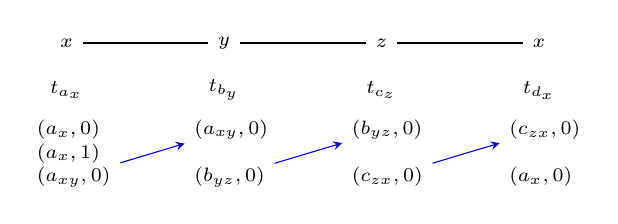
\begin{tikzpicture}
    \node (x1) at (0,0) {\scriptsize $x$};
    \node (y) at (2, 0) {\scriptsize $y$};
    \node (z) at (4, 0) {\scriptsize $z$};
    \node (x2) at (6, 0) {\scriptsize $x$};
    \draw [thin] (x1) to (y) to (z) to (x2);

    \begin{scope}[yshift=-0.6cm]
    \node (a) at (0,0) {\scriptsize $t_{a_x}$};
    \node (b) at (2, 0) {\scriptsize $t_{b_y}$};
    \node (c) at (4, 0) {\scriptsize $t_{c_z}$};
    \node (d) at (6, 0) {\scriptsize $t_{d_x}$};
    %\draw [thin] (a) to (b) to (c) to (d);

    \node [right] at (-0.5, -0.5) {\scriptsize $\wt(a_x, 0)$};
    \node [right] at (-0.5, -0.8) {\scriptsize $\wt(a_x, 1)$};
    \node [right] (1) at (-0.5, -1.1) {\scriptsize $\wt(a_{xy}, 0)$};

    \node [right] (2) at (1.5, -0.5) {\scriptsize $\rd(a_{xy}, 0)$};
    \node [right] (3) at (1.5, -1.1) {\scriptsize $\wt(b_{yz}, 0)$};

    \draw [blue, ->, >=stealth] (1) to  (2);

    \node [right] (4) at (3.5, -0.5) {\scriptsize $\rd(b_{yz}, 0)$};
    \node [right] (5) at (3.5, -1.1) {\scriptsize $\wt(c_{zx}, 0)$};
    \draw [blue, ->, >=stealth] (3) to  (4);

    \node [right] (6) at (5.5, -0.5) {\scriptsize $\rd(c_{zx}, 0)$};
    \node [right] (7) at (5.5, -1.1) {\scriptsize $\rd(a_x, 0)$};
    \draw [blue, ->, >=stealth] (5) to  (6);

    \end{scope}
  \end{tikzpicture}
  }  
  \caption{From triangles to violations of weak-read-coherence} 
  \label{fig:super-linear-illustration}
\end{figure}

Our idea for the reduction is as follows. We will construct $\expartial$ in such a way that for every $\rd(x, v)$ there is a unique $\wt(x, v)$ present in the entire program. Therefore, the $\rf$ relation is fixed. If $G$ has a triangle, we will have a shared variable $a$ and a cycle of the form: $\wt(a, 0) \xrightarrow{\po} \wt(a, 1) \xrightarrow{\hb} \rd(a, 0) \xrightarrow{\rf^{-1}} \wt(a, 0)$. This cycle violates weak-read-coherence.
If $\expartial$ with the fixed $\rf$ violates  
\WRCoh{}, then $G$ has a triangle.  The $\hb$ path $\wt(a, 1) \xrightarrow{\hb} \rd(a, 0)$ should reflect the presence of a triangle in $G$. Here is the full construction.

%The key aspect of the construction is depicted in Figure~\ref{fig:super-linear-illustration}. Suppose $G$ contains a triangle over vertices $x, y, z$. We consider a variable $a_x$ for which we extract an $\hb$ path as above. To force the $\hb$ path to have length $3$, we consider four copies $t_{a_x}, t_{b_x}, t_{c_x}, t_{d_x}$ for each vertex $x$. When there is edge $(x, y)$, thread $t_{a_x}$ writes to $t_{b_y}$. Similarly, $(y, z)$ makes $t_{b_y}$ write to $t_{c_z}$ and finally the edge $(z, x)$ makes $t_{c_z}$ write to $t_{d_x}$ which contains $\rd(a_x, 0)$. Here is the full Construction. 

\noindent{\bf{Construction}}. Given an undirected graph $G = (V_G, E_G)$ with $n$ vertices, we construct a partial execution graph $\expartial = \tup{\E, \po}$ with $|\E|=\mathcal{O}(V_G+E_G)$ such that $\expartial$ satisfies weak-read-coherence iff $G$ is triangle-free.
For simplicity, we let $V_G=\{1,\dots, n\}$. As the graph is undirected, we assume that if $(u,v) \in E$ then $(v, u) \in E$.

\smallskip 
\noindent \emph{Events, threads  and memory locations}. For each  vertex $v \in V_G$, we have threads $t_{a_v}, t_{b_v}, t_{c_v}$ and $t_{d_v}$. 
For each edge $(u,v) \in E_G$, we have locations $a_{uv}, b_{uv}, c_{uv}$. We also have locations $a_v, b_v, c_v$ for $v \in V_G$. 
The events are $\wt(a_v,0), \wt(a_v,1), \rd(a_v, 0)$, as well as $\{\wt(x_{uv},0), \rd(x_{uv},0) \mid x \in \{a,b,c\}\}$. 
We also have events $\wt(b_v),\wt(c_v)$ (the values do not matter).  
This gives us $4|V_G|$ threads, $3(|E_G|+|V_G|)$ locations and $5|V_G|+2|E_G|$ events. 

We now describe the threads. 
Let $v \in V_G$ and $x \in \{a,b, c\}$. Let $N_v=\{\alpha \mid (v, \alpha) \in E_G\}$.
Let $W(x_{vw},0), R(x_{vw},0)$ be  macros representing respectively, 
the sequence of events $\wt(x_{v\alpha_1},0) \dots \wt(x_{v\alpha_m},0)$ 
and $\rd(x_{v\alpha_1},0) \dots \rd(x_{v\alpha_m},0)$ such that 
$\alpha_1, \dots, \alpha_n \in N_v$. 

\begin{align*}
& t_{a_v}: \wt(a_v,0) \wt(a_v,1) W(a_{vw},0) \\
& t_{b_v}: R(a_{wv},0) ~w(b_v)~ W(b_{vw},0) \\
& t_{c_v}: R(b_{wv},0)~w(c_v)~W(c_{vw},0) \\
& t_{d_v}: R(c_{wv},0)\rd(a_v,0)
\end{align*}


The construction is such that each location is written into by a unique thread. Further, each location is accessed only by at most two threads. Each location (barring $a_v$) is written into exactly once by its writer thread and the $\rf$ is trivially determined. Thus, the constructed $\expartial$ qualifies as a single writer. 
The construction has the following properties. 
\begin{enumerate}
    \item $(x, y) \in E_G$ iff $\wt(a_{x},0)~\po~\wt(a_{x},1)~\hb~\wt(b_{y})$
    \item $(x, y) \in E_G$ iff $\wt(b_{x})~\hb~\wt(c_{y})$
    \item $(x, y) \in E_G$ iff $\wt(c_{x})~\hb~\rd(a_{y},0)$
\end{enumerate}


Thus, a path $x-y-z$ of length 2 results in $\wt(a_x,1)~\po~\wt(a_x,0)~\hb~\wt(b_y)~\hb~\wt(c_z)$, and  a
path $x-y-z-w$ of length 3 results in 
\[\wt(a_x,1)~\po~\wt(a_x,0)~\hb~\wt(b_y)~\hb~\wt(c_z)~\hb~\rd(a_w,0) \]

The key invariant behind the reduction is that for any $v \in V_G$, $\wt(a_v,1)~ \hb ~\rd(a_v,0)$ iff $G$ contains a triangle. The former 
violates weak-read-coherence. Figure \ref{fig:super-linear-lower-bound} shows the reduction on a graph with 3 vertices $\{1,2,3\}$, having edges between every distinct pair of vertices.  




\begin{figure*}[!htbp]
\newcommand{\xtstep}{0.3}
\newcommand{\ytstep}{0.7}
\newcommand{\ybias}{-0.3 }
\newcommand{\xstep}{1.4}
\newcommand{\ystep}{-0.6}
\newcommand{\xtscale}{0.8}
\def\crossoutopacity{0.3}
\def \numevents{5}
\def\scale{0.73}
\centering
\scalebox{\scale}{
\begin{tikzpicture}[thick,font=\footnotesize,
pre/.style={<-,shorten >= 2pt, shorten <=2pt, very thick},
post/.style={->,shorten >= 3pt, shorten <=3pt,   thick},
seqtrace/.style={line width=1},
und/.style={very thick, draw=gray},
virt/.style={circle,draw=black!50,fill=black!20, opacity=0}]
\tikzstyle{event} = [rectangle, fill=white, inner sep=0, minimum height=4.6mm, minimum width=14mm, rounded corners]

\node[] (S11) at (-5.5*\xstep,.1) {\normalsize $t_{a_1}$};
\node[] (S12) at (-5.5*\xstep,\numevents * \ystep) {};
\node[] (S21) at (-4.5*\xstep,.1) {\normalsize $t_{a_2}$};
\node[] (S22) at (-4.5*\xstep,\numevents * \ystep) {};
\node[] (S31) at (-3.5*\xstep,.1) {\normalsize $t_{a_3}$};
\node[] (S32) at (-3.5*\xstep,\numevents * \ystep) {};
\node[] (S41) at (-2.5*\xstep,.1) {\normalsize $t_{b_1}$};
\node[] (S42) at (-2.5*\xstep,\numevents * \ystep) {};
\node[] (S51) at (-1.5*\xstep,.1) {\normalsize $t_{b_2}$};
\node[] (S52) at (-1.5*\xstep,\numevents * \ystep) {};
\node[] (S61) at (-.5*\xstep,.1) {\normalsize $t_{b_3}$};
\node[] (S62) at (-.5*\xstep,\numevents * \ystep) {};
\node[] (S71) at (.5*\xstep,.1) {\normalsize $t_{c_1}$};
\node[] (S72) at (.5*\xstep,\numevents * \ystep) {};
\node[] (S81) at (1.5*\xstep,.1) {\normalsize $t_{c_2}$};
\node[] (S82) at (1.5*\xstep,\numevents * \ystep) {};
\node[] (S91) at (2.5*\xstep,.1) {\normalsize $t_{c_3}$};
\node[] (S92) at (2.5*\xstep,\numevents * \ystep) {};
\node[] (S101) at (3.5*\xstep,.1) {\normalsize $t_{d_1}$};
\node[] (S102) at (3.5*\xstep,\numevents * \ystep) {};
\node[] (S111) at (4.5*\xstep,.1) {\normalsize $t_{d_2}$};
\node[] (S112) at (4.5*\xstep,\numevents * \ystep) {};
\node[] (S121) at (5.5*\xstep,.1) {\normalsize $t_{d_3}$};
\node[] (S122) at (5.5*\xstep,\numevents * \ystep) {};



\draw[seqtrace] (S11) to (S12);
\draw[seqtrace] (S21) to (S22);
\draw[seqtrace] (S31) to (S32);
\draw[seqtrace] (S41) to (S42);
\draw[seqtrace] (S51) to (S52);
\draw[seqtrace] (S61) to (S62);
\draw[seqtrace] (S71) to (S72);
\draw[seqtrace] (S81) to (S82);
\draw[seqtrace] (S91) to (S92);
\draw[seqtrace] (S101) to (S102);
\draw[seqtrace] (S111) to (S112);
\draw[seqtrace] (S121) to (S122);




\node[event] (11) at (-5.5*\xstep, 1*\ystep + 0*\ybias) {$\wt(a_1,0)$};
\node[event] (12) at (-5.5*\xstep, 2*\ystep + 0*\ybias) {$\wt(a_1,1)$};
\node[event] (13) at (-5.5*\xstep, 3*\ystep + 0*\ybias) {$\wt(a_{12},0)$};
\node[event] (14) at (-5.5*\xstep, 4*\ystep + 0*\ybias) {$\wt(a_{13},0)$};



\node[event] (11) at (-4.5*\xstep, 1*\ystep + 0*\ybias) {$\wt(a_2,0)$};
\node[event] (12) at (-4.5*\xstep, 2*\ystep + 0*\ybias) {$\wt(a_2,1)$};
\node[event] (13) at (-4.5*\xstep, 3*\ystep + 0*\ybias) {$\wt(a_{21},0)$};
\node[event] (14) at (-4.5*\xstep, 4*\ystep + 0*\ybias) {$\wt(a_{23},0)$};



\node[event] (11) at (-3.5*\xstep, 1*\ystep + 0*\ybias) {$\wt(a_3,0)$};
\node[event] (12) at (-3.5*\xstep, 2*\ystep + 0*\ybias) {$\wt(a_3,1)$};
\node[event] (13) at (-3.5*\xstep, 3*\ystep + 0*\ybias) {$\wt(a_{31},0)$};
\node[event] (14) at (-3.5*\xstep, 4*\ystep + 0*\ybias) {$\wt(a_{32},0)$};

\node[event] (11) at (-2.5*\xstep, 1*\ystep + 0*\ybias) {$\rd(a_{31},0)$};
\node[event] (12) at (-2.5*\xstep, 2*\ystep + 0*\ybias) {$\rd(a_{21},0)$};
\node[event] (12) at (-2.5*\xstep, 3*\ystep + 0*\ybias) {$\wt(b_1)$};
\node[event] (13) at (-2.5*\xstep, 4*\ystep + 0*\ybias) {$\wt(b_{12},0)$};
\node[event] (14) at (-2.5*\xstep, 5*\ystep + 0*\ybias) {$\wt(b_{13},0)$};



\node[event] (11) at (-1.5*\xstep, 1*\ystep + 0*\ybias) {$\rd(a_{32},0)$};
\node[event] (12) at (-1.5*\xstep, 2*\ystep + 0*\ybias) {$\rd(a_{12},0)$};
\node[event] (12) at (-1.5*\xstep, 3*\ystep + 0*\ybias) {$\wt(b_2)$};
\node[event] (13) at (-1.5*\xstep, 4*\ystep + 0*\ybias) {$\wt(b_{21},0)$};
\node[event] (14) at (-1.5*\xstep, 5*\ystep + 0*\ybias) {$\wt(b_{23},0)$};

\node[event] (11) at (-.5*\xstep, 1*\ystep + 0*\ybias) {$\rd(a_{23},0)$};
\node[event] (12) at (-.5*\xstep, 2*\ystep + 0*\ybias) {$\rd(a_{13},0)$};
\node[event] (12) at (-.5*\xstep, 3*\ystep + 0*\ybias) {$\wt(b_3)$};
\node[event] (13) at (-.5*\xstep, 4*\ystep + 0*\ybias) {$\wt(b_{31},0)$};
\node[event] (14) at (-.5*\xstep, 5*\ystep + 0*\ybias) {$\wt(b_{32},0)$};


\node[event] (11) at (.5*\xstep, 1*\ystep + 0*\ybias) {$\rd(b_{31},0)$};
\node[event] (12) at (.5*\xstep, 2*\ystep + 0*\ybias) {$\rd(b_{21},0)$};
\node[event] (12) at (.5*\xstep, 3*\ystep + 0*\ybias) {$\wt(c_1)$};
\node[event] (13) at (.5*\xstep, 4*\ystep + 0*\ybias) {$\wt(c_{12},0)$};
\node[event] (14) at (.5*\xstep, 5*\ystep + 0*\ybias) {$\wt(c_{13},0)$};


\node[event] (11) at (1.5*\xstep, 1*\ystep + 0*\ybias) {$\rd(b_{32},0)$};
\node[event] (12) at (1.5*\xstep, 2*\ystep + 0*\ybias) {$\rd(b_{12},0)$};
\node[event] (12) at (1.5*\xstep, 3*\ystep + 0*\ybias) {$\wt(c_2)$};
\node[event] (13) at (1.5*\xstep, 4*\ystep + 0*\ybias) {$\wt(c_{21},0)$};
\node[event] (14) at (1.5*\xstep, 5*\ystep + 0*\ybias) {$\wt(c_{23},0)$};


\node[event] (11) at (2.5*\xstep, 1*\ystep + 0*\ybias) {$\rd(b_{23},0)$};
\node[event] (12) at (2.5*\xstep, 2*\ystep + 0*\ybias) {$\rd(b_{13},0)$};
\node[event] (12) at (2.5*\xstep, 3*\ystep + 0*\ybias) {$\wt(c_3)$};
\node[event] (13) at (2.5*\xstep, 4*\ystep + 0*\ybias) {$\wt(c_{31},0)$};
\node[event] (14) at (2.5*\xstep, 5*\ystep + 0*\ybias) {$\wt(c_{32},0)$};


\node[event] (11) at (3.5*\xstep, 1*\ystep + 0*\ybias) {$\rd(c_{31},0)$};
\node[event] (12) at (3.5*\xstep, 2.5*\ystep + 0*\ybias) {$\rd(c_{21},0)$};
\node[event] (13) at (3.5*\xstep, 4*\ystep + 0*\ybias) {$\rd(a_{1},0)$};

\node[event] (11) at (4.5*\xstep, 1*\ystep + 0*\ybias) {$\rd(c_{32},0)$};
\node[event] (12) at (4.5*\xstep, 2.5*\ystep + 0*\ybias) {$\rd(c_{12},0)$};
\node[event] (13) at (4.5*\xstep, 4*\ystep + 0*\ybias) {$\rd(a_{2},0)$};

\node[event] (11) at (5.5*\xstep, 1*\ystep + 0*\ybias) {$\rd(c_{23},0)$};
\node[event] (12) at (5.5*\xstep, 2.5*\ystep + 0*\ybias) {$\rd(c_{13},0)$};
\node[event] (13) at (5.5*\xstep, 4*\ystep + 0*\ybias) {$\rd(a_{3},0)$};

\end{tikzpicture}
}
\caption{
A partial execution $\expartial$ for a graph $G=(\{1,2,3\}, \{(1,2), (2,1),(1,3), (3,1), (2,3), (3,2)\})$. 
We have $(\wt(a_1,0), \rd(a_1,0))\in \hb$  violating weak read coherence in $\expartial$.
\label{fig:super-linear-lower-bound}
}
\end{figure*}

\noindent{\bf{Correctness and Time Complexity}}. Assume that $G$ has a triangle $(x, y, z)$. Wlg, let $x < y < z$. Then $\wt(a_x,1) ~\hb~ \rd(a_x,0)$ as follows: 
$\wt(a_x,1) ~\po ~\wt(a_{xy},0)$ $~\rf~ \rd(a_{xy},0)~\po~\wt(b_{yz},0)~\rf ~$ $\rd(b_{yz},0)~\po~\wt(c_{zx},0)~\rf~\rd(c_{zx},0)~\po~\rd(a_x,0)$ (See Figure~\ref{fig:super-linear-illustration}). 
Together with $\wt(a_x,0)~\po~\wt(a_x,1)$, we obtain a weak-read-coherence violation. 
 Triangle-freeness in the input graph $G$ ensures satisfying weak-read-coherence. In the construction, the only way to violate weak-read-coherence 
is to have $\wt(a_v,0)~\po~\wt(a_v,1)~\hb ~\rd(a_v,0)$ for some $v \in V_G$. This is achieved by:
\[ \wt(a_v,1)~\po~\wt(a_{vu},0)~\hb~\wt(b_{uw},0)~\hb~\wt(c_{wv},0)~\rf~\rd(c_{wv},0)~\po~\rd(a_v,0)\] 

This points to a triangle $v u w$ in $G$.   
The total time to construct $\expartial$ is $O(V_G+E_G)$. 
\smallskip

We have seen how the special structure of $\onewriter$ systems eliminates the combinatorial problem of synthesizing $\mo$, since the writes to each location are already totally ordered by program order. This  makes the $\vm$ problem polynomial time for $\ramm$ and its variants. On the other hand the conditional lower bound suggests that the algorithm cannot be faster than detecting triangles in a graph. The next chapter will be dedicated to hardness results for multi-writers discussed in the beginning of this chapter. 

